%% Unit 5: Fabrication Laboratory
%% Included from main.tex via %% Unit 5: Fabrication Laboratory
%% Included from main.tex via %% Unit 5: Fabrication Laboratory
%% Included from main.tex via %% Unit 5: Fabrication Laboratory
%% Included from main.tex via \include{./units/unit5}
%% Requires the macros/colours defined in main.tex's preamble.

%==============================================================================
\section{Fabrication Laboratory}
%==============================================================================
\unitdivider{V}{Fabrication Laboratory}{The route map: survey to service blueprint}

\begin{frame}{The Fab-Lab Route Map}
  \begin{columns}[c]
    \begin{column}{0.5\textwidth}
      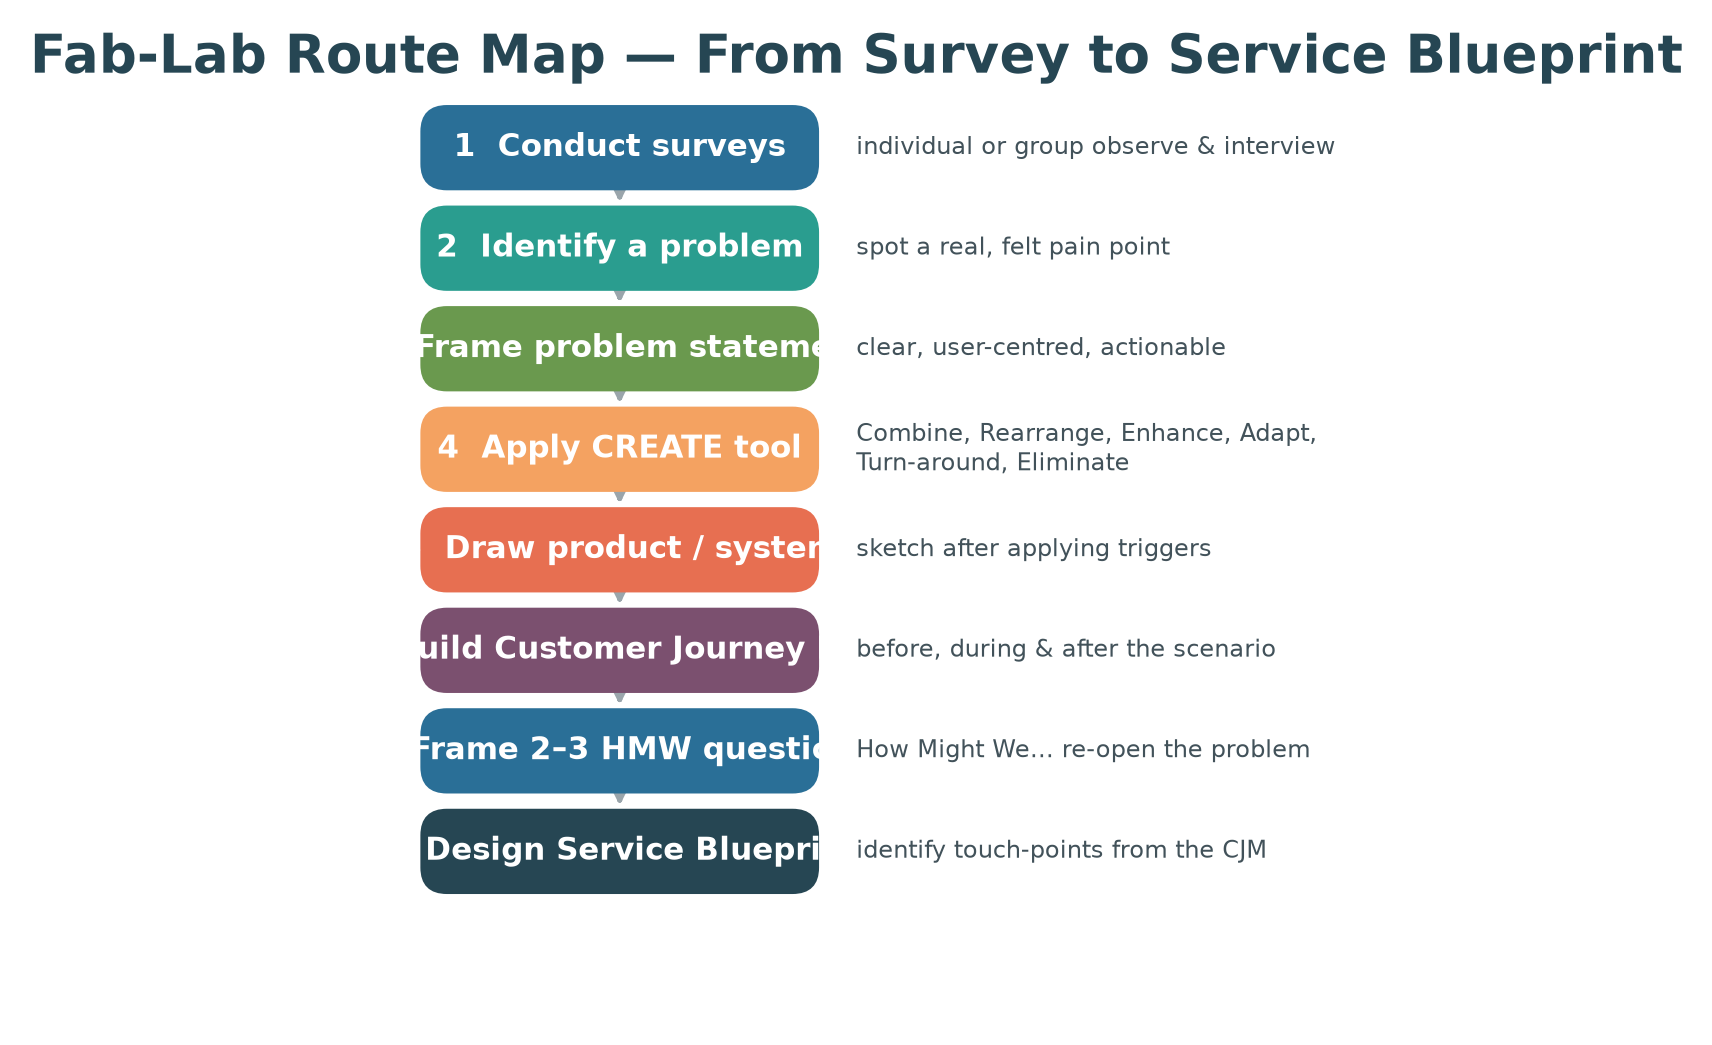
\includegraphics[width=\linewidth]{figures/route_map.png}
    \end{column}
    \begin{column}{0.5\textwidth}\scriptsize
      A step-by-step recipe for the lab project:
      \begin{enumerate}\scriptsize
        \item Conduct surveys.
        \item Identify a problem.
        \item Frame a problem statement.
        \item Apply the \kwt{CREATE} tool.
        \item Draw the product / system.
        \item Build a Customer Journey Map.
        \item Frame 2--3 \kwt{HMW} questions.
        \item Design a Service Blueprint.
      \end{enumerate}
    \end{column}
  \end{columns}
\end{frame}

\begin{frame}{Surveys, Problems \& Problem Statements}
  \accentrule\\[0.3em]
  \begin{columns}[T]
    \begin{column}{0.5\textwidth}\small
      \textbf{Conduct surveys}
      \begin{itemize}\small
        \item Individually or as a group.
        \item Observe, interview, question.
        \item Look for \kwc{real, felt pains}.
      \end{itemize}
      \textbf{Identify a problem} worth solving.
    \end{column}
    \begin{column}{0.5\textwidth}
      \begin{block}{Framing a problem statement}\scriptsize
        A good statement is \kwt{user-centred}, \kwt{clear} and
        \kwt{actionable}:\\[0.3em]
        \emph{"[User] needs [need] because [insight]."}\\[0.3em]
        Avoid baking in a solution — describe the \emph{problem}.
      \end{block}
    \end{column}
  \end{columns}
\end{frame}

\begin{frame}{The CREATE Tool}
  \begin{columns}[c]
    \begin{column}{0.55\textwidth}
      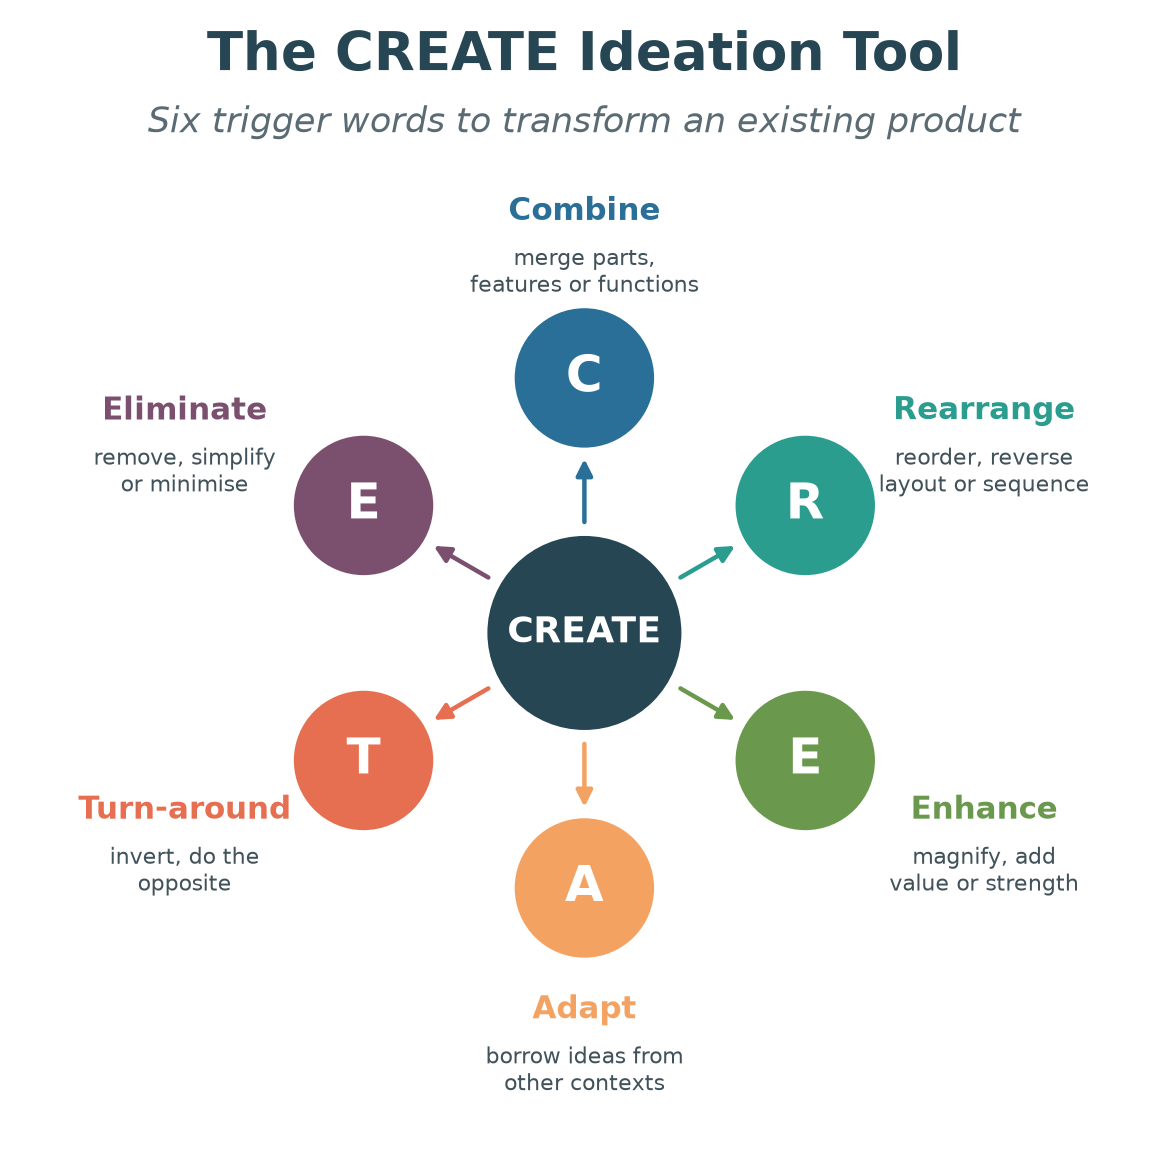
\includegraphics[width=\linewidth]{figures/create_tool.png}
    \end{column}
    \begin{column}{0.45\textwidth}\scriptsize
      \kw{CREATE} is a set of \emph{trigger words} to transform an existing
      product:
      \begin{itemize}\scriptsize
        \item \textbf{C}ombine \quad \textbf{R}earrange
        \item \textbf{E}nhance \quad \textbf{A}dapt
        \item \textbf{T}urn-around \quad \textbf{E}liminate
      \end{itemize}
      \vspace{0.3em}
      Apply each trigger to your problem, then \kwt{draw the product / system}
      that results.
    \end{column}
  \end{columns}
\end{frame}

\begin{frame}{Customer Journey Map (CJM)}
  \bigfig{cjm.png}{Map actions, touch-points, emotions \& pain points — before, during \& after.}
\end{frame}

\begin{frame}{How Might We (HMW) Questions}
  \begin{columns}[c]
    \begin{column}{0.55\textwidth}
      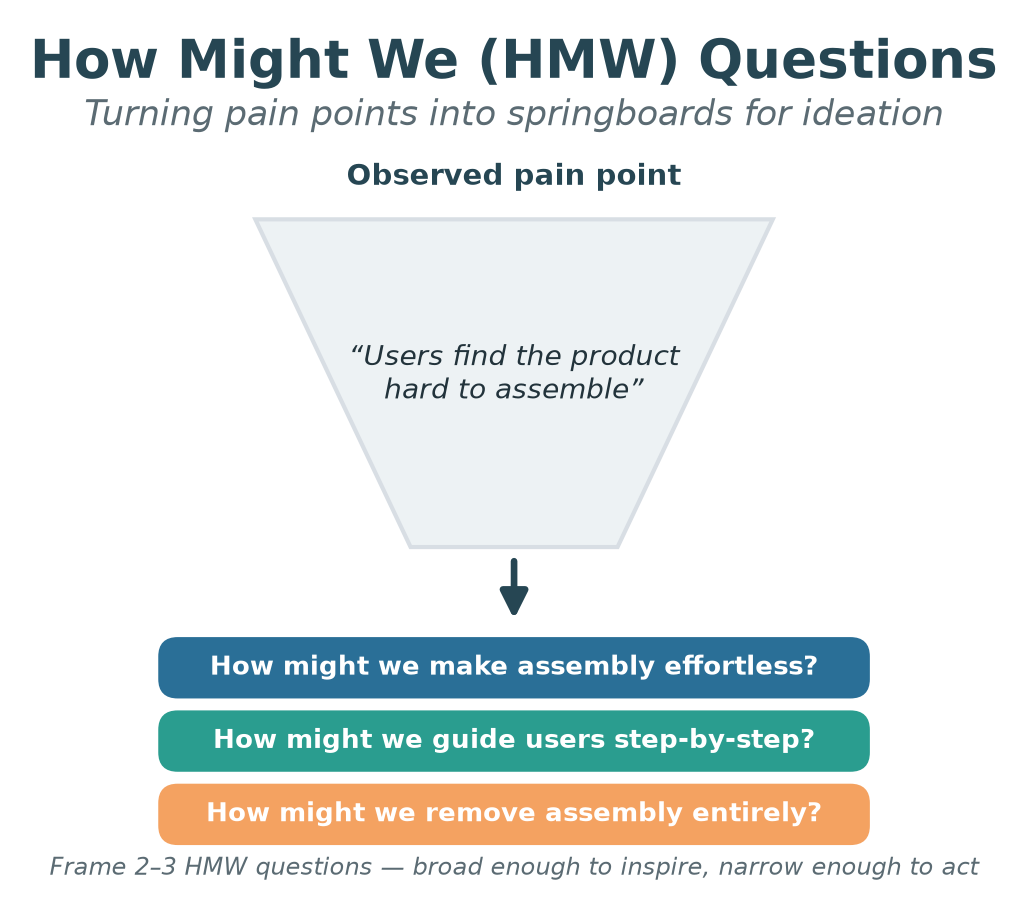
\includegraphics[width=\linewidth]{figures/hmw.png}
    \end{column}
    \begin{column}{0.45\textwidth}\scriptsize
      Turn each \kwc{pain point} from the CJM into an optimistic
      \kw{"How Might We\ldots"} question.
      \vspace{0.3em}
      \begin{itemize}\scriptsize
        \item Broad enough to \emph{inspire} ideas.
        \item Narrow enough to \emph{act} on.
        \item Frame \textbf{2--3} for your mock scenario.
      \end{itemize}
    \end{column}
  \end{columns}
\end{frame}

\begin{frame}{Service Blueprint}
  \bigfig{service_blueprint.png}{Layer the journey with front-stage, back-stage \& support processes; identify touch-points.}
\end{frame}

%% Requires the macros/colours defined in main.tex's preamble.

%==============================================================================
\section{Fabrication Laboratory}
%==============================================================================
\unitdivider{V}{Fabrication Laboratory}{The route map: survey to service blueprint}

\begin{frame}{The Fab-Lab Route Map}
  \begin{columns}[c]
    \begin{column}{0.5\textwidth}
      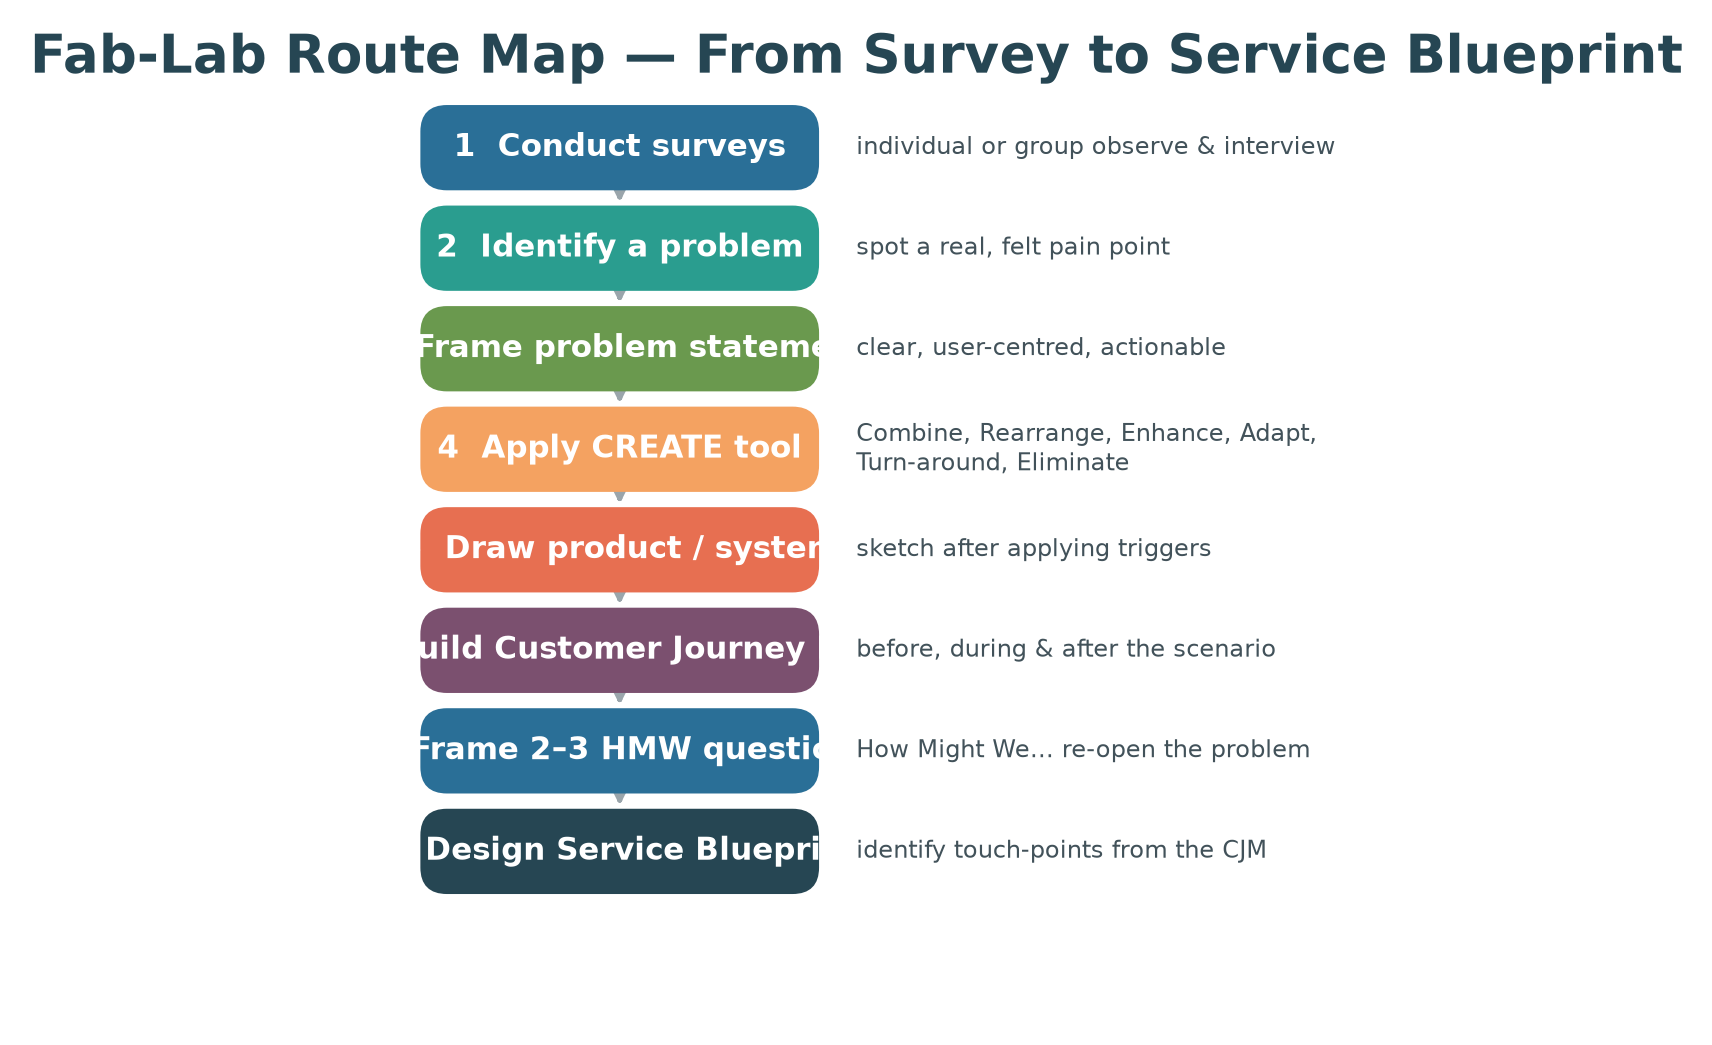
\includegraphics[width=\linewidth]{figures/route_map.png}
    \end{column}
    \begin{column}{0.5\textwidth}\scriptsize
      A step-by-step recipe for the lab project:
      \begin{enumerate}\scriptsize
        \item Conduct surveys.
        \item Identify a problem.
        \item Frame a problem statement.
        \item Apply the \kwt{CREATE} tool.
        \item Draw the product / system.
        \item Build a Customer Journey Map.
        \item Frame 2--3 \kwt{HMW} questions.
        \item Design a Service Blueprint.
      \end{enumerate}
    \end{column}
  \end{columns}
\end{frame}

\begin{frame}{Surveys, Problems \& Problem Statements}
  \accentrule\\[0.3em]
  \begin{columns}[T]
    \begin{column}{0.5\textwidth}\small
      \textbf{Conduct surveys}
      \begin{itemize}\small
        \item Individually or as a group.
        \item Observe, interview, question.
        \item Look for \kwc{real, felt pains}.
      \end{itemize}
      \textbf{Identify a problem} worth solving.
    \end{column}
    \begin{column}{0.5\textwidth}
      \begin{block}{Framing a problem statement}\scriptsize
        A good statement is \kwt{user-centred}, \kwt{clear} and
        \kwt{actionable}:\\[0.3em]
        \emph{"[User] needs [need] because [insight]."}\\[0.3em]
        Avoid baking in a solution — describe the \emph{problem}.
      \end{block}
    \end{column}
  \end{columns}
\end{frame}

\begin{frame}{The CREATE Tool}
  \begin{columns}[c]
    \begin{column}{0.55\textwidth}
      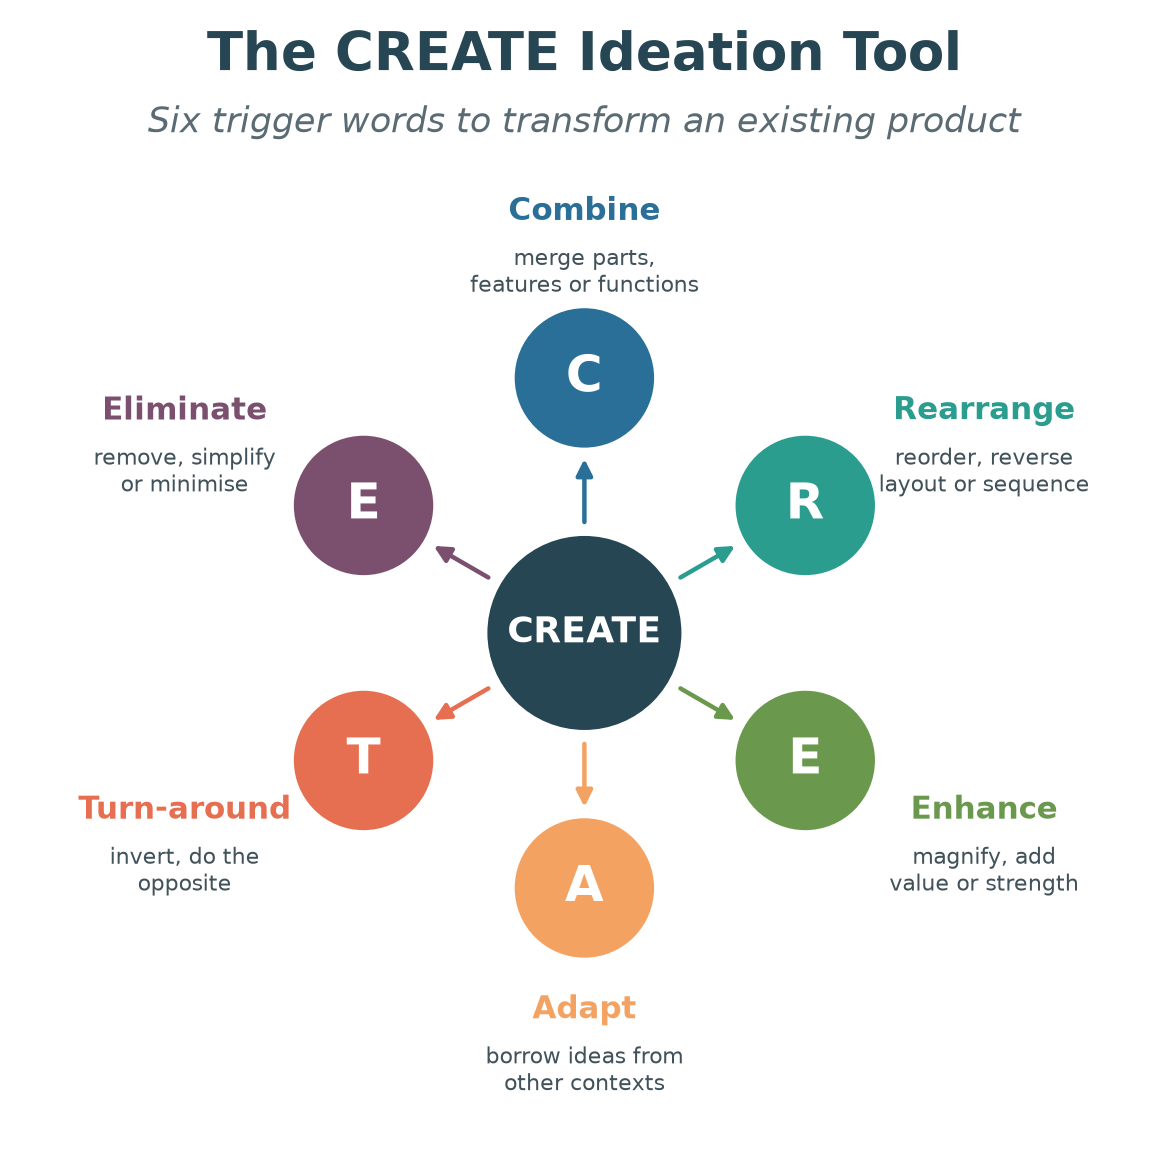
\includegraphics[width=\linewidth]{figures/create_tool.png}
    \end{column}
    \begin{column}{0.45\textwidth}\scriptsize
      \kw{CREATE} is a set of \emph{trigger words} to transform an existing
      product:
      \begin{itemize}\scriptsize
        \item \textbf{C}ombine \quad \textbf{R}earrange
        \item \textbf{E}nhance \quad \textbf{A}dapt
        \item \textbf{T}urn-around \quad \textbf{E}liminate
      \end{itemize}
      \vspace{0.3em}
      Apply each trigger to your problem, then \kwt{draw the product / system}
      that results.
    \end{column}
  \end{columns}
\end{frame}

\begin{frame}{Customer Journey Map (CJM)}
  \bigfig{cjm.png}{Map actions, touch-points, emotions \& pain points — before, during \& after.}
\end{frame}

\begin{frame}{How Might We (HMW) Questions}
  \begin{columns}[c]
    \begin{column}{0.55\textwidth}
      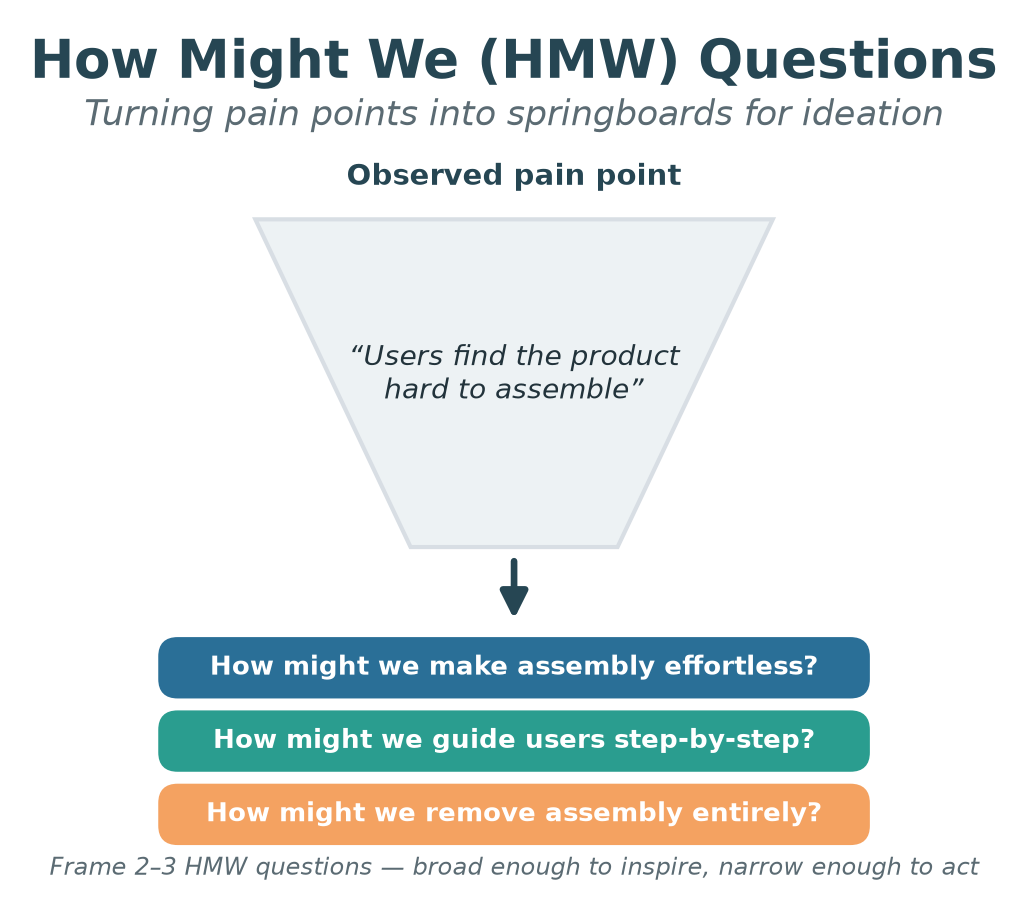
\includegraphics[width=\linewidth]{figures/hmw.png}
    \end{column}
    \begin{column}{0.45\textwidth}\scriptsize
      Turn each \kwc{pain point} from the CJM into an optimistic
      \kw{"How Might We\ldots"} question.
      \vspace{0.3em}
      \begin{itemize}\scriptsize
        \item Broad enough to \emph{inspire} ideas.
        \item Narrow enough to \emph{act} on.
        \item Frame \textbf{2--3} for your mock scenario.
      \end{itemize}
    \end{column}
  \end{columns}
\end{frame}

\begin{frame}{Service Blueprint}
  \bigfig{service_blueprint.png}{Layer the journey with front-stage, back-stage \& support processes; identify touch-points.}
\end{frame}

%% Requires the macros/colours defined in main.tex's preamble.

%==============================================================================
\section{Fabrication Laboratory}
%==============================================================================
\unitdivider{V}{Fabrication Laboratory}{The route map: survey to service blueprint}

\begin{frame}{The Fab-Lab Route Map}
  \begin{columns}[c]
    \begin{column}{0.5\textwidth}
      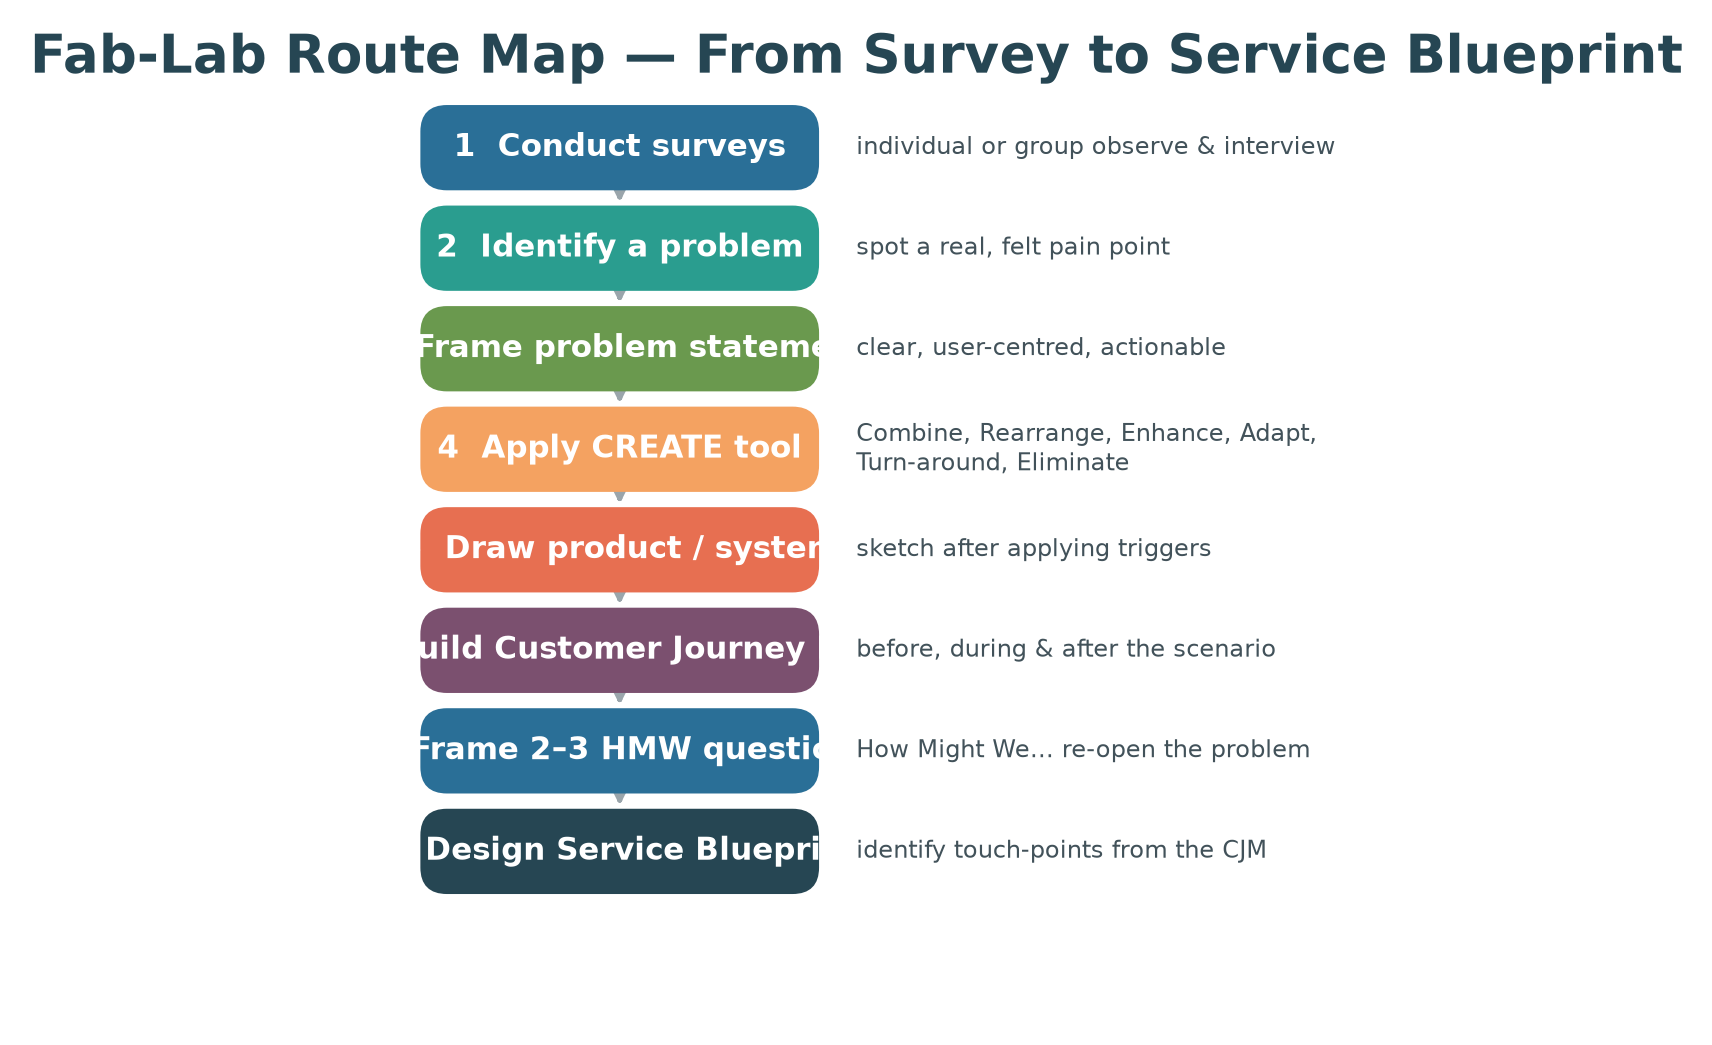
\includegraphics[width=\linewidth]{figures/route_map.png}
    \end{column}
    \begin{column}{0.5\textwidth}\scriptsize
      A step-by-step recipe for the lab project:
      \begin{enumerate}\scriptsize
        \item Conduct surveys.
        \item Identify a problem.
        \item Frame a problem statement.
        \item Apply the \kwt{CREATE} tool.
        \item Draw the product / system.
        \item Build a Customer Journey Map.
        \item Frame 2--3 \kwt{HMW} questions.
        \item Design a Service Blueprint.
      \end{enumerate}
    \end{column}
  \end{columns}
\end{frame}

\begin{frame}{Surveys, Problems \& Problem Statements}
  \accentrule\\[0.3em]
  \begin{columns}[T]
    \begin{column}{0.5\textwidth}\small
      \textbf{Conduct surveys}
      \begin{itemize}\small
        \item Individually or as a group.
        \item Observe, interview, question.
        \item Look for \kwc{real, felt pains}.
      \end{itemize}
      \textbf{Identify a problem} worth solving.
    \end{column}
    \begin{column}{0.5\textwidth}
      \begin{block}{Framing a problem statement}\scriptsize
        A good statement is \kwt{user-centred}, \kwt{clear} and
        \kwt{actionable}:\\[0.3em]
        \emph{"[User] needs [need] because [insight]."}\\[0.3em]
        Avoid baking in a solution — describe the \emph{problem}.
      \end{block}
    \end{column}
  \end{columns}
\end{frame}

\begin{frame}{The CREATE Tool}
  \begin{columns}[c]
    \begin{column}{0.55\textwidth}
      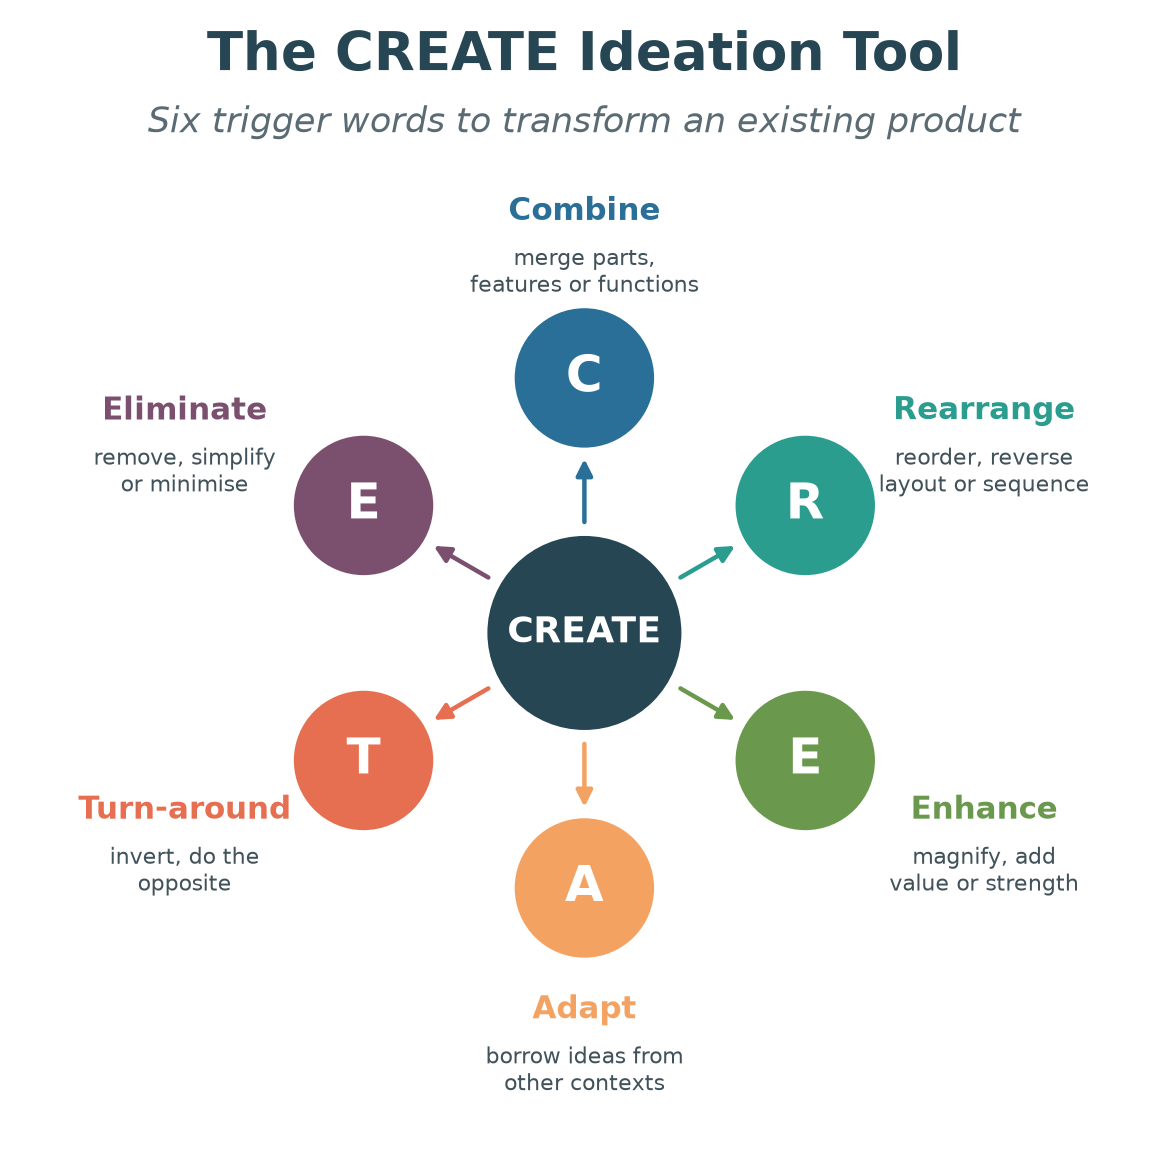
\includegraphics[width=\linewidth]{figures/create_tool.png}
    \end{column}
    \begin{column}{0.45\textwidth}\scriptsize
      \kw{CREATE} is a set of \emph{trigger words} to transform an existing
      product:
      \begin{itemize}\scriptsize
        \item \textbf{C}ombine \quad \textbf{R}earrange
        \item \textbf{E}nhance \quad \textbf{A}dapt
        \item \textbf{T}urn-around \quad \textbf{E}liminate
      \end{itemize}
      \vspace{0.3em}
      Apply each trigger to your problem, then \kwt{draw the product / system}
      that results.
    \end{column}
  \end{columns}
\end{frame}

\begin{frame}{Customer Journey Map (CJM)}
  \bigfig{cjm.png}{Map actions, touch-points, emotions \& pain points — before, during \& after.}
\end{frame}

\begin{frame}{How Might We (HMW) Questions}
  \begin{columns}[c]
    \begin{column}{0.55\textwidth}
      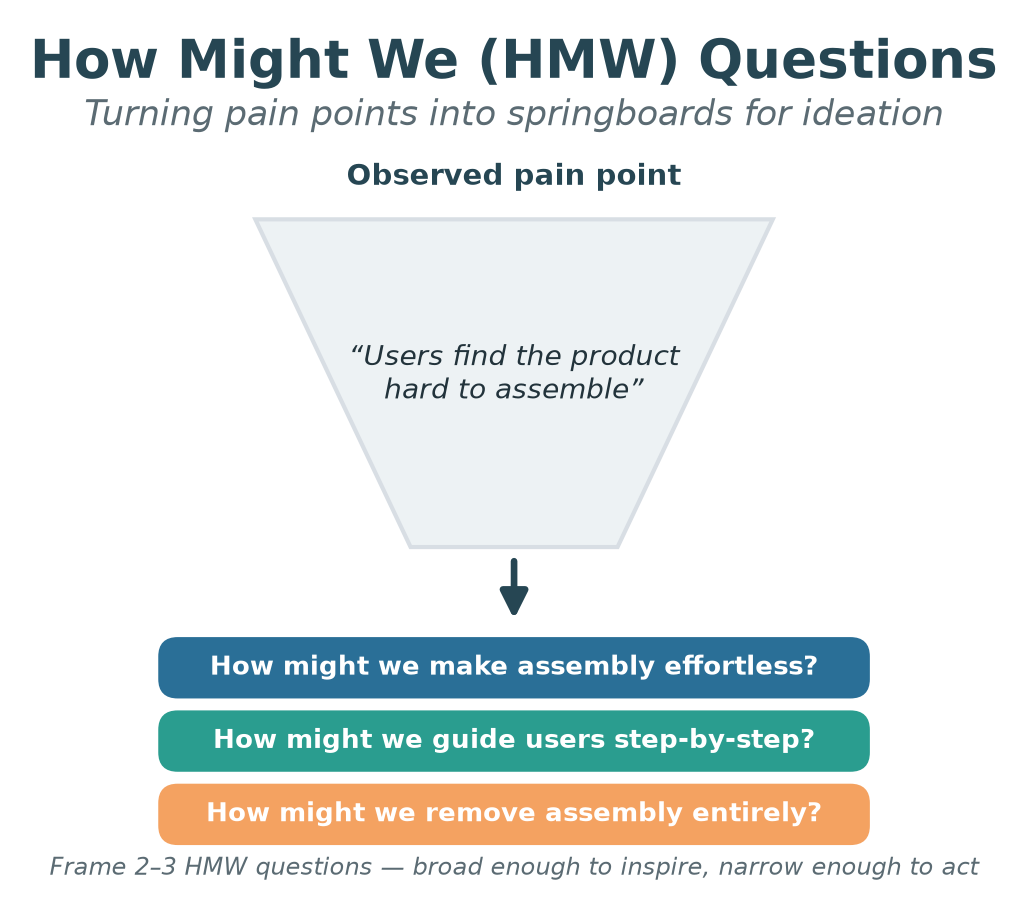
\includegraphics[width=\linewidth]{figures/hmw.png}
    \end{column}
    \begin{column}{0.45\textwidth}\scriptsize
      Turn each \kwc{pain point} from the CJM into an optimistic
      \kw{"How Might We\ldots"} question.
      \vspace{0.3em}
      \begin{itemize}\scriptsize
        \item Broad enough to \emph{inspire} ideas.
        \item Narrow enough to \emph{act} on.
        \item Frame \textbf{2--3} for your mock scenario.
      \end{itemize}
    \end{column}
  \end{columns}
\end{frame}

\begin{frame}{Service Blueprint}
  \bigfig{service_blueprint.png}{Layer the journey with front-stage, back-stage \& support processes; identify touch-points.}
\end{frame}

%% Requires the macros/colours defined in main.tex's preamble.

%==============================================================================
\section{Fabrication Laboratory}
%==============================================================================
\unitdivider{V}{Fabrication Laboratory}{The route map: survey to service blueprint}

\begin{frame}{The Fab-Lab Route Map}
  \begin{columns}[c]
    \begin{column}{0.5\textwidth}
      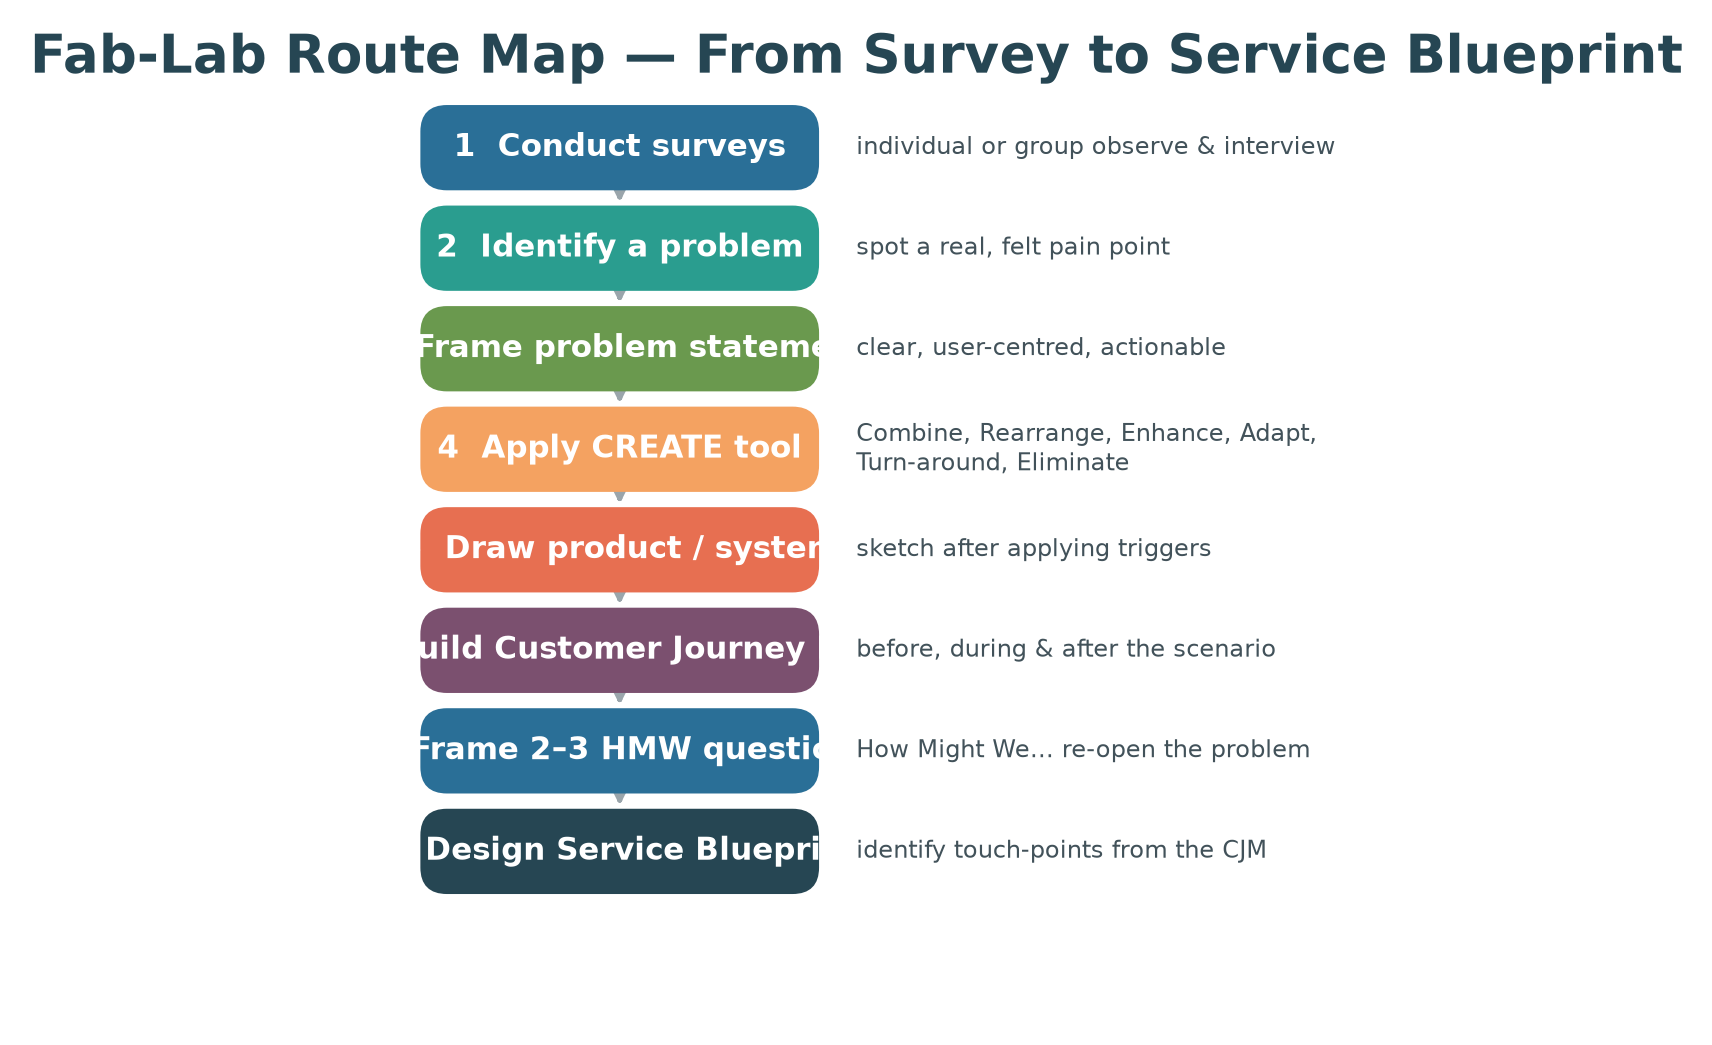
\includegraphics[width=\linewidth]{figures/route_map.png}
    \end{column}
    \begin{column}{0.5\textwidth}\scriptsize
      A step-by-step recipe for the lab project:
      \begin{enumerate}\scriptsize
        \item Conduct surveys.
        \item Identify a problem.
        \item Frame a problem statement.
        \item Apply the \kwt{CREATE} tool.
        \item Draw the product / system.
        \item Build a Customer Journey Map.
        \item Frame 2--3 \kwt{HMW} questions.
        \item Design a Service Blueprint.
      \end{enumerate}
    \end{column}
  \end{columns}
\end{frame}

\begin{frame}{Surveys, Problems \& Problem Statements}
  \accentrule\\[0.3em]
  \begin{columns}[T]
    \begin{column}{0.5\textwidth}\small
      \textbf{Conduct surveys}
      \begin{itemize}\small
        \item Individually or as a group.
        \item Observe, interview, question.
        \item Look for \kwc{real, felt pains}.
      \end{itemize}
      \textbf{Identify a problem} worth solving.
    \end{column}
    \begin{column}{0.5\textwidth}
      \begin{block}{Framing a problem statement}\scriptsize
        A good statement is \kwt{user-centred}, \kwt{clear} and
        \kwt{actionable}:\\[0.3em]
        \emph{"[User] needs [need] because [insight]."}\\[0.3em]
        Avoid baking in a solution — describe the \emph{problem}.
      \end{block}
    \end{column}
  \end{columns}
\end{frame}

\begin{frame}{The CREATE Tool}
  \begin{columns}[c]
    \begin{column}{0.55\textwidth}
      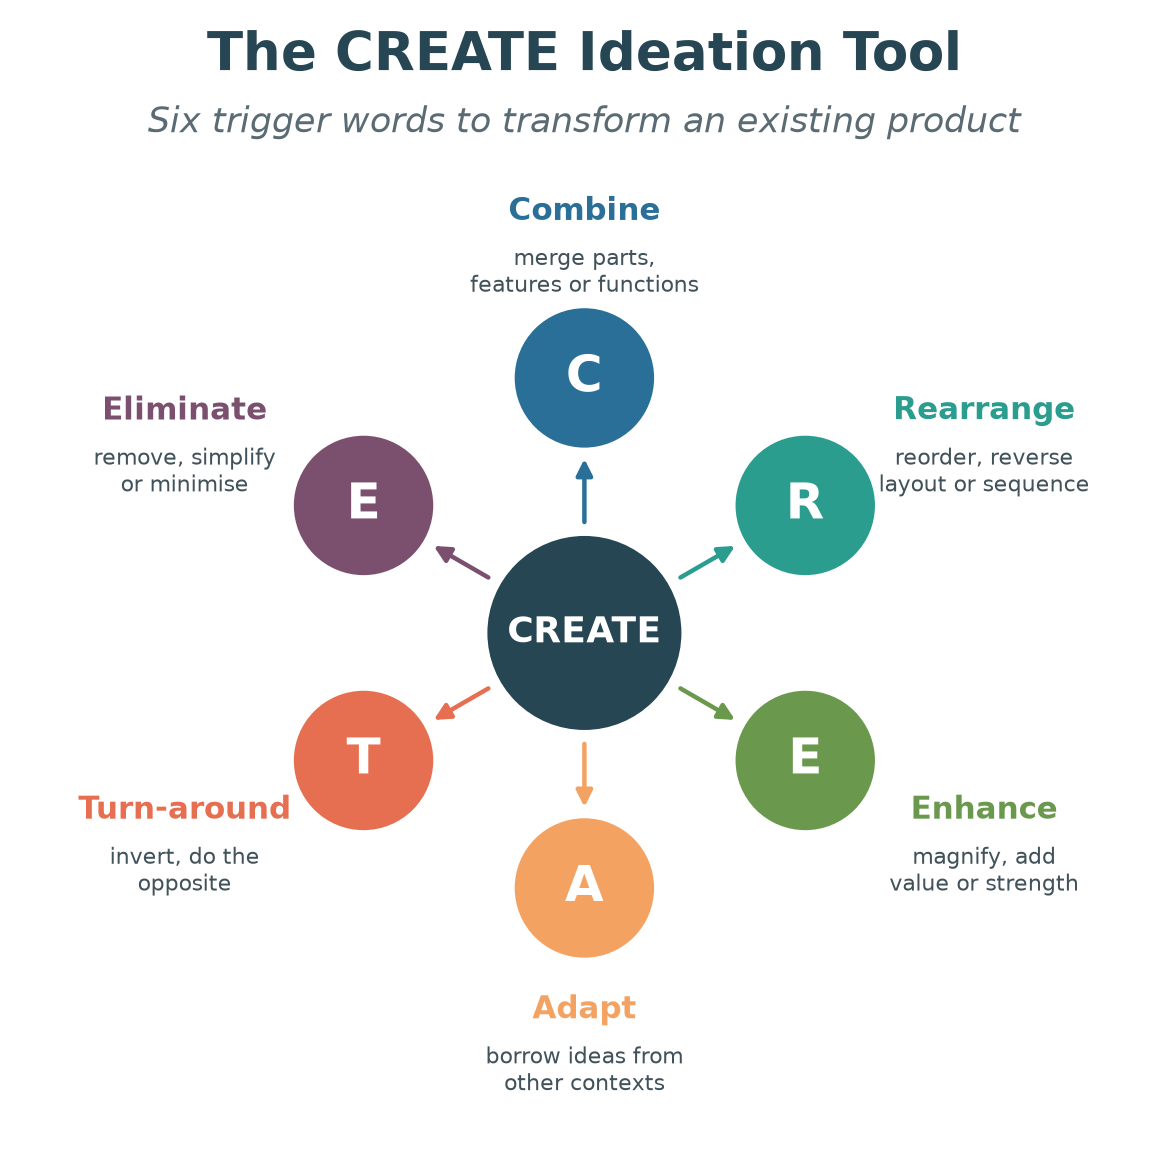
\includegraphics[width=\linewidth]{figures/create_tool.png}
    \end{column}
    \begin{column}{0.45\textwidth}\scriptsize
      \kw{CREATE} is a set of \emph{trigger words} to transform an existing
      product:
      \begin{itemize}\scriptsize
        \item \textbf{C}ombine \quad \textbf{R}earrange
        \item \textbf{E}nhance \quad \textbf{A}dapt
        \item \textbf{T}urn-around \quad \textbf{E}liminate
      \end{itemize}
      \vspace{0.3em}
      Apply each trigger to your problem, then \kwt{draw the product / system}
      that results.
    \end{column}
  \end{columns}
\end{frame}

\begin{frame}{Customer Journey Map (CJM)}
  \bigfig{cjm.png}{Map actions, touch-points, emotions \& pain points — before, during \& after.}
\end{frame}

\begin{frame}{How Might We (HMW) Questions}
  \begin{columns}[c]
    \begin{column}{0.55\textwidth}
      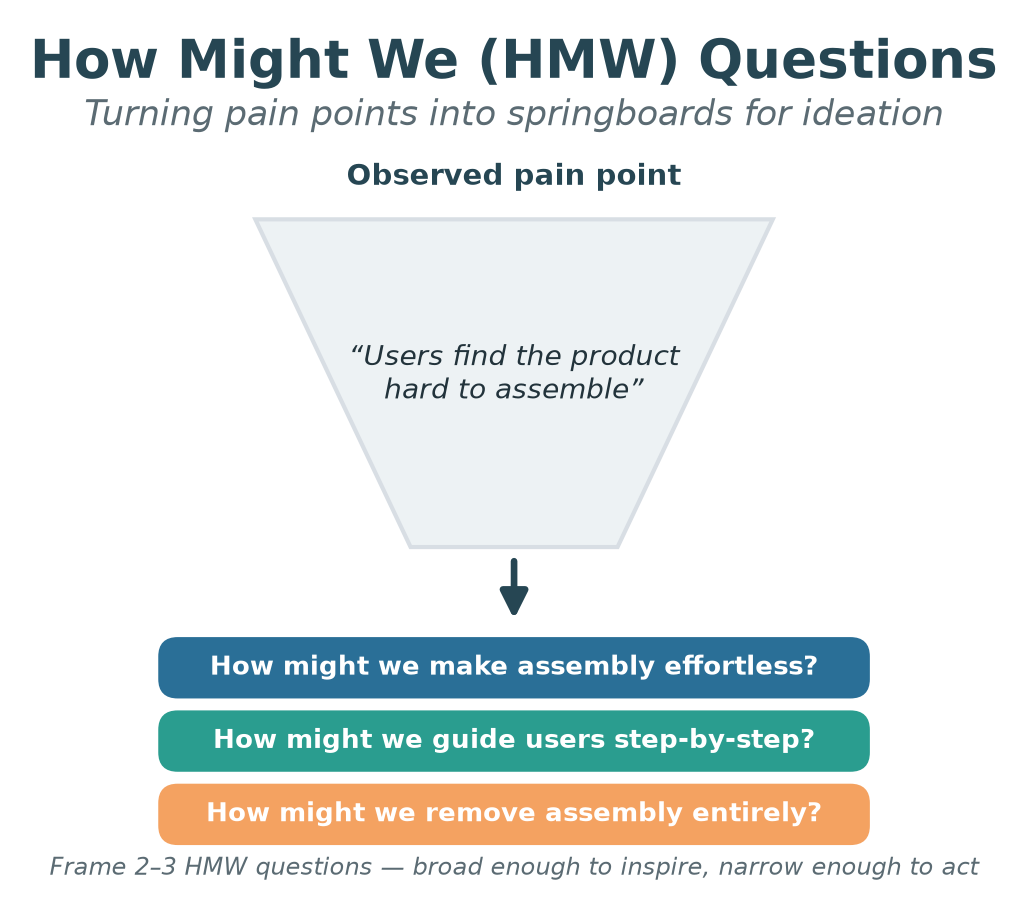
\includegraphics[width=\linewidth]{figures/hmw.png}
    \end{column}
    \begin{column}{0.45\textwidth}\scriptsize
      Turn each \kwc{pain point} from the CJM into an optimistic
      \kw{"How Might We\ldots"} question.
      \vspace{0.3em}
      \begin{itemize}\scriptsize
        \item Broad enough to \emph{inspire} ideas.
        \item Narrow enough to \emph{act} on.
        \item Frame \textbf{2--3} for your mock scenario.
      \end{itemize}
    \end{column}
  \end{columns}
\end{frame}

\begin{frame}{Service Blueprint}
  \bigfig{service_blueprint.png}{Layer the journey with front-stage, back-stage \& support processes; identify touch-points.}
\end{frame}
